% !TEX root = ../thesis_main.tex

\section{BSA as a prolate ellipsoid}
\graphicspath{{rom_studies/figs/}}

The crystal structure of the BSA (pdb 4f5s) used in our simulations corresponds
to a dimer. Knowing that this structure can be modeled as an ellipsoid \cite{SquireETal1968},
we look for different alternatives to decide the dimensions of the ellipsoid. We took two
different approaches, a surface model and a volume model. The first attempt is 
the surface model which consists on finding the dimensions
of an ellipsoid that encapsules all the charges within the protein. We determined the principal axes of this
ellipsoid using Principal Component Analysis. Principal component analysis is a technique that
uses orthogonal transformations and brings out patterns in a set of data. When 
we use a PCA in three dimensions, these transformations ensure that the first 
component is the one with most variation, the second one is the second-most, and
third one the least. This technique provided us the three eigenvectors that best 
describe the cloud of mesh-vertices. The values of the principal axis are $a=98.9\, \text{\AA}$, $b=54.2\, \text{\AA}$, and $c=41.8\, \text{\AA}$. 
Using these vectors when creating the mesh of the ellipsoid ensures that all the charges are contained.
The second approach to model the BSA is to create an ellipsoid that matches the volume of the BSA. To find the dimensions 
of the volume-equivalent equivalent we made some approximations. We obtained the volume of the BSA protein original mesh
using Trimesh (\url{https://github.com/mikedh/trimesh})), and looking at the PCA principal axis we notice that $b$ and $c$ are close 
compared to $a$, then $b=c=x$ and $a$ is double the size $a=2x$. Using these approximations we can write the volume of the ellipsoid:

\begin{equation}
    V_e = \frac{4\pi}{3}a\,b\,c 
\end{equation}

as 

\begin{equation}
    V_e = \frac{4\pi}{3}2\,x^3
\end{equation}

Knowing that the volume of the volume of the BSA protein is $V_e = 166642 \, \text{\AA}^3$ we get that $x=27.09496 \, \text{\AA}$ 
and therefore $a=54.18993 \, \text{\AA}$ and $b=c=27.09496 \, \text{\AA}$. These dimensions give us an ellipsoid that hast the same volume 
as the original BSA mesh, however, we can not encapsule all the charges inside of it. To be able to use this model we needed to study first the 
effects of replacing the distribution of charges by a monopole, as well as the possibility of not include them in the model. 

\subsection{Effect of presence of charges}

Since the PCA model can encapsuled all the charges we intended to use this model to study the effect of using the charges distribution, versus
a monopole representation of the charges ("center of mass"), and also no charges present. To ensure that we are solving the equations properly, 
we perform a convergence analysis.


\subsubsection{PCA ellipsoid convergence analysis}

We performed a grid convergence analysis on the PCA (Principal component analysis) ellipsoid - sensor system containing a full pqr (see Figure \ref{fig:one_pca_sketch}). 
Since we compute the extinction cross section of the sensor (8 nm radius silver sphere), we set a fixed mesh density for the ellipsoid and refine 
the mesh of the sphere ($N=512, 2048, 8192, 32768$). We found that a mesh with $N=5120$ elements for the ellipsoid was fine enough for the convergence analysis.
We used the same physical conditions and parameters that were used for the BSA-nanoparticle convergence analysis presented in
\ref{sec:grid_conv_bsa}. Similarly to the BSA-sensor system, the distance between the sensor and the PCA-ellipsoid 
was $d=1$ nm, and the ellipsoid was oriented such that the dipole moment of the charges was aligned with the $y$-axis. To obtain the error 
estimate we used Richardson extrapolated value of the extinction cross section as a reference, $C_{ext} = 1432.6560$ nm$^2$.
The observed order of convergence is $0.99$, and Figure \ref{fig:err_sph-pca} shows that the error decays with the number of boundary elements ($1/N$). This provides
evidence that the numerical solutions computed with \pygbe are correctly resolved by the meshes.  Table \ref{table:err_sph-pca} shows the percentages error for the different 
meshes used in this study.

\begin{figure}%[h] %  figure placement: here, top, bottom, or page
    \centering
    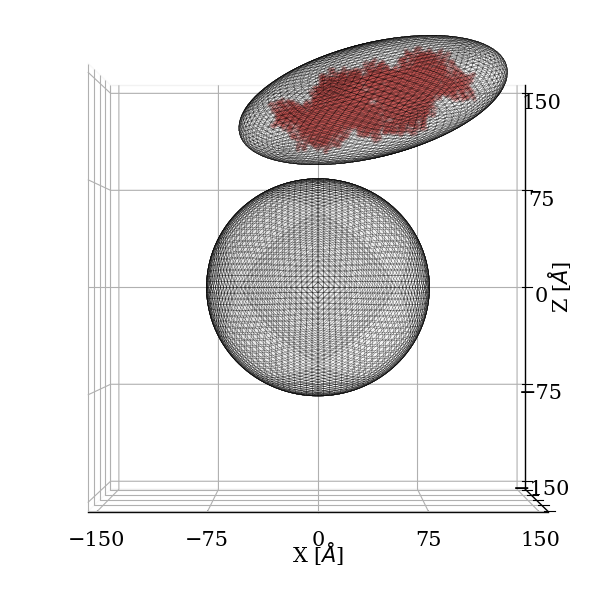
\includegraphics[width=0.65\textwidth]{viz/one_pca_full_display.png} 
    \caption{Sensor protein display: PCA ellipsoid with charges distribution located at $\pm 1$ nm of the 
    nanoparticle in the $z$-direction.}
    \label{fig:one_pca_sketch}
 \end{figure}


\begin{figure}%[h] %  figure placement: here, top, bottom, or page
    \centering
    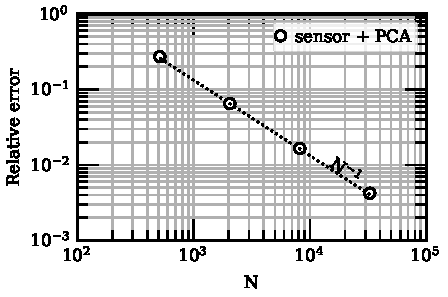
\includegraphics[width=0.85\textwidth]{convergence_sensor_pca_w380.pdf} 
    \caption{Grid-convergence study of extinction cross-section of a spherical silver
             nanoparticle with a PCA ellipsoid at $d=1$ nm which contains 
             the charges distribution within it.}
    \label{fig:err_sph-pca}
 \end{figure}

 \begin{table}%[h]
    \centering
    \caption{\label{table:err_sph-pca} Estimated percentage error of the PCA ellipsoid-sensor 
    system, with respect to the extrapolated value 
    (using Richardson extrapolation).} 
    \begin{tabular}{c c}
    \hline%\toprule
    N & \% error \\
    \hline%\midrule
     $512$ & $27.2$ \\
     $2048$ & $6.5$ \\
     $8192$ & $1.66$ \\
     $32768$ & $0.42$ \\
    \hline%\bottomrule
    \end{tabular}
\end{table}

After performing the convergence analysis studies, we relaxed the numerical parameters of the computations to reduce the run-time without 
compromising accuracy. The following parameters were used to obtain non-convergence results presented from now on for the case of PCA ellipsoids.

\begin{table}%[h]
    \centering
    \caption{\label{table:rel_pca_par} Relaxed parameters for the PCA ellipsoid case. The parameters that are not 
    mentioned here remain the same as in the convergence study.} 
    \begin{tabular}{c c}
    \hline%\toprule
    parameter & \% value \\
    \hline%\midrule
     $N_{snesor}$ & $8192$ \\
     $k_{fine}$ & $19$ \\
     $P$ & $6$ \\
     $tol$ & $1\times 10^{-3}$ \\
    \hline%\bottomrule
    \end{tabular}
\end{table}

The Richardson extrapolated value for the PCA case is: $1432.6561$ nm$^2$ and the computed value with the relaxed parameters 
is $1456.0781$ nm$^2$. If we compute the percentage error we obtain $1.63 \%$.

\subsubsection{Charges model analysis}

In order to know if we could use a VE approach we needed to study the effect of the charges. We analyze
the different representations of pqr (full distribution and equivalent monopole) as well as the impact of having
no charges present. The setup of the simulations consist in a silver sphere sensor ($r=8$ nm) with a PCA ellipsoid 
at 1 nm of the surface of the sensor in the $z$-direction, oriented such that the dipole moment is aligned with the $y$-axis. We run 
three different cases, one with the full charges distribution, a second case with one equivalent charge located in the
"center of mass", and lastly an empty ellipsoid with no charges. Figure \ref{fig:pqr_pca} shows the results for the different models of the 
charge distribution as well as the results when there are no charges present within the ellipsoid. 


\begin{figure}%[h] %  figure placement: here, top, bottom, or page
    \centering
    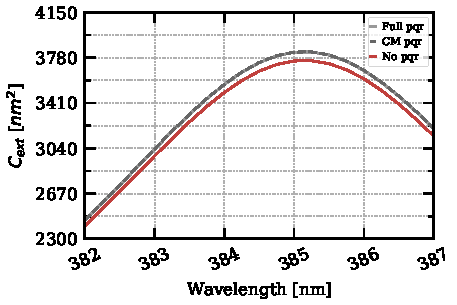
\includegraphics[width=0.85\textwidth]{pqr_analysis_pca.pdf} 
    \caption{Extinction cross-section as a function of wavelength for an $8$ nm
    silver sphere immersed in water with one PCA ellipsoid at $1$ nm away from 
    the surface in the $z$-direction, under a constant electric field on the $z$-direction.
    The label "Full pqr" corresponds to the full distribution of charges, the label "CM pqr" corresponds to a monopole representation 
    of the charges obtained by computing the center of mass of them, and the label "No pqr" 
    corresponds to the case where there are no charges present.}
    \label{fig:pqr_pca}
 \end{figure}

 The maximum value for all the curves in Figure \ref{fig:pqr_pca} occurs at $385.25$ nm. The 
 maximum value of the extinction cross section for the full distribution ("Full pqr") is $3827.06$ nm$^2$ and for 
 the monopole/center-of-mass representation ("CM pqr") is $3828.21$ nm$^2$, what results in a difference of $0.03 \,\%$. The
 maximum value of the extinction cross section when there are no charges present ("No pqr") is $3755.51$ nm$^2$ which compared to 
 the maximum for the full distribution gives us a difference of $1.87 \,\%$. Looking at these results we can say that the presence of 
 charges inside the protein does not affect the wavelength shift. However, it does affect the intensity of the maximum value of the 
 extinction cross section by approximately $2 \,\%$. Finally, we can say that using a monopole approximation for the distribution of charges, 
 is equivalent to using teh full distribution of charges.
